\documentclass[aspectratio=169,10pt]{beamer}

\usetheme{Madrid}
\usecolortheme{seahorse}
\setbeamertemplate{navigation symbols}{}
\setbeamertemplate{footline}[frame number]

\usepackage{booktabs}
\usepackage{amsmath}
\usepackage{graphicx}
\usepackage{xcolor}
\usepackage{tikz}
\usetikzlibrary{arrows.meta, positioning, shapes.geometric, calc}

% Custom colors
\definecolor{umblue}{RGB}{0,39,76}
\definecolor{ummaize}{RGB}{255,203,5}
\definecolor{todocolor}{RGB}{220,50,50}
\definecolor{lightgray}{RGB}{240,240,240}
\definecolor{gpuA40}{RGB}{70,130,180}
\definecolor{gpuA100}{RGB}{60,179,113}
\definecolor{gpuH100}{RGB}{255,140,0}
\definecolor{gpuV100}{RGB}{169,169,169}
\definecolor{gpuL40S}{RGB}{148,103,189}

\setbeamercolor{title}{fg=umblue}
\setbeamercolor{frametitle}{fg=umblue}

\newcommand{\todo}[1]{\textcolor{todocolor}{\textbf{[TODO: #1]}}}

\title[cp.async Cross-GPU Study]{Predicting \texttt{cp.async} Pipeline Effectiveness\\from Memory-Subsystem Parameters:\\A Cross-GPU Study}
\author{Xiangchen Song \quad Chenxin Geng \quad Yuyang Feng \quad Tian Xia}
\institute{EECS 570 -- Parallel Computer Architecture \\ University of Michigan}
\date{Milestone 1 \quad March 18, 2026}

\begin{document}

% ============================================================
% Slide 1: Title
% ============================================================
\begin{frame}
\titlepage
\end{frame}

% ============================================================
% Slide 2: Problem & Motivation
% ============================================================
\begin{frame}{Problem \& Motivation}

\begin{columns}[T]
\begin{column}{0.55\textwidth}
\textbf{Background:}
\begin{itemize}
    \item NVIDIA \texttt{cp.async} (Ampere+) enables asynchronous global$\to$shared memory copies, overlapping with computation
    \item CUTLASS, FlashAttention-3, Triton all rely on multi-stage \texttt{cp.async} pipelines; pipeline depth $S$ is a key tuning knob
\end{itemize}

\vspace{0.5em}
\textbf{The Problem:}
\begin{itemize}
    \item Practitioners tune $S$ on \emph{one} GPU and assume it transfers
    \item But pipeline effectiveness depends on \textbf{L2 capacity}, \textbf{memory BW/latency}, and \textbf{per-SM shared memory} --- which vary \emph{dramatically} across GPUs
    \item No existing autotuner uses architecture parameters to prune the search space
\end{itemize}
\end{column}

\begin{column}{0.42\textwidth}
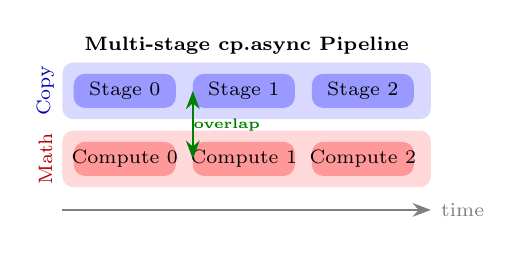
\begin{tikzpicture}[scale=0.72, every node/.style={font=\scriptsize}]
    % cp.async pipeline diagram
    \fill[blue!15, rounded corners] (0,3.2) rectangle (6.5,4.2);
    \fill[red!15, rounded corners]  (0,2.0) rectangle (6.5,3.0);

    \node[font=\scriptsize\bfseries] at (3.25,4.5) {Multi-stage cp.async Pipeline};

    % Stage labels
    \foreach \i/\label in {0/Stage 0, 1/Stage 1, 2/Stage 2} {
        \fill[blue!40, rounded corners] (0.2+\i*2.1, 3.4) rectangle (2.0+\i*2.1, 4.0);
        \node at (1.1+\i*2.1, 3.7) {\label};
    }
    \foreach \i/\label in {0/Compute 0, 1/Compute 1, 2/Compute 2} {
        \fill[red!40, rounded corners] (0.2+\i*2.1, 2.2) rectangle (2.0+\i*2.1, 2.8);
        \node at (1.1+\i*2.1, 2.5) {\label};
    }

    \node[font=\scriptsize, blue!70!black] at (-0.3, 3.7) [rotate=90] {Copy};
    \node[font=\scriptsize, red!70!black]  at (-0.3, 2.5) [rotate=90] {Math};

    \draw[-{Stealth}, thick, gray] (0,1.6) -- (6.5,1.6) node[right] {time};

    % Overlap arrow
    \draw[{Stealth}-{Stealth}, thick, green!50!black] (2.3,2.5) -- (2.3,3.7);
    \node[green!50!black, font=\tiny\bfseries] at (2.9,3.1) {overlap};
\end{tikzpicture}

\vspace{0.3em}
\begin{block}{\small Research Question}
\scriptsize Does optimal $S^*$ and its speedup diverge across GPUs with different memory subsystems? Can a parameter-free model predict this?
\end{block}
\end{column}
\end{columns}
\end{frame}

% ============================================================
% Slide 3: Hypotheses
% ============================================================
\begin{frame}{Three Falsifiable Hypotheses}

\renewcommand{\arraystretch}{1.3}
\begin{table}
\centering
\scriptsize
\begin{tabular}{@{}p{1.8cm} p{4.5cm} p{6.5cm}@{}}
\toprule
\textbf{Hypothesis} & \textbf{Core Mechanism} & \textbf{Falsifiable Prediction} \\
\midrule
\textbf{H1}\newline L2-capacity\newline driven
  & Speedup inflects when $W_{\text{conc}} > C_{\text{L2}}$; L2-normalized curves collapse onto one master curve
  & After normalization, A100-MIG (20\,MiB) and H100 (50\,MB) should \emph{not} overlap --- if they do despite $2.4\times$ L2 gap, H1 is insufficient \\
\midrule
\textbf{H2}\newline Ridge-point\newline driven
  & Speedup governed by ridge point $R = F_{\text{peak}}/\text{BW}_{\text{peak}}$; low-$R$ GPUs benefit most
  & Speedup ordering: A100-MIG ($R{=}7.9$) $>$ H100 ($R{=}20$) $>$ A40 ($R{=}53.7$). \emph{Not} correlated with L2 size \\
\midrule
\textbf{H3}\newline Latency--\newline occupancy\newline tension
  & Optimal $S^*$ balances DRAM latency (deeper $\to$ better) vs.\ SMEM pressure (deeper $\to$ worse occupancy)
  & $S^*(N)$ is \emph{non-monotonic} on A40 (high latency + small SMEM); monotone/flat on A100-MIG and H100 \\
\bottomrule
\end{tabular}
\end{table}

\vspace{0.3em}
\centering
\small In practice, a \textbf{mixture} is likely --- the predictive model incorporates all three mechanisms.

\end{frame}

% ============================================================
% Slide 4: Hardware Setup
% ============================================================
\begin{frame}{Experimental Setup: Hardware}

\begin{columns}[T]
\begin{column}{0.58\textwidth}
\renewcommand{\arraystretch}{1.15}
\begin{table}
\centering
\scriptsize
\begin{tabular}{@{}lccccc@{}}
\toprule
 & \textcolor{gpuV100}{\textbf{V100}} & \textcolor{gpuA40}{\textbf{A40}} & \textcolor{gpuA100}{\textbf{A100 MIG}} & \textcolor{gpuL40S}{\textbf{L40S}} & \textcolor{gpuH100}{\textbf{H100}} \\
\midrule
Arch       & Volta  & Ampere & Ampere    & Ada    & Hopper \\
SMs        & 80     & 84     & 42        & 142    & 132 \\
\texttt{cp.async} & ---  & \checkmark & \checkmark & \checkmark & \checkmark \\
Memory     & HBM2   & GDDR6  & HBM2e     & GDDR6  & HBM3 \\
Peak BW    & 900    & 696    & 968       & 864    & 3350\,GB/s \\
L2 (nominal) & 6\,MB  & 6\,MB  & 20\,MiB & 96\,MB & 50\,MB \\
L2 (measured) & ---  & 8\,MB  & TBD       & 112\,MB & 28\,MB \\
SMEM/SM    & 96\,KB & 100\,KB & 164\,KB  & 100\,KB & 228\,KB \\
FP32 peak  & 15.7   & 37.4   & 7.6       & 45.7   & 67\,TF \\
\textbf{Ridge}  & 17.4   & \textbf{53.7}  & \textbf{7.9} & 52.9 & 20.0 \\
\midrule
Role & Boundary & \multicolumn{2}{c}{Core contrast} & L2 extreme & Core anchor \\
\bottomrule
\end{tabular}
\end{table}
\end{column}

\begin{column}{0.40\textwidth}
\textbf{Design rationale:}
\begin{itemize}\scriptsize
    \item \textbf{A40 vs H100}: max memory-subsystem gap ($8.3\times$ L2, $4.8\times$ BW)
    \item \textbf{A100 MIG}: lowest ridge (7.9) $\to$ H2 predicts most benefit; tests MIG
    \item \textbf{L40S}: largest L2 (96\,MB nominal, 112\,MB measured) $\to$ tests ``L2 absorbs all'' extreme
    \item \textbf{V100}: no \texttt{cp.async} $\to$ boundary condition ($1.0\times$)
\end{itemize}

\vspace{0.3em}
\scriptsize
\textbf{Key finding:} Measured L2 $\neq$ nominal L2. H100 nominal 50\,MB $\to$ effective 28\,MB (L2 slicing); L40S nominal 96\,MB $\to$ effective 112\,MB.
\end{column}
\end{columns}
\end{frame}

% ============================================================
% Slide 5: Kernels & Methodology
% ============================================================
\begin{frame}{Experimental Setup: Kernels \& Methodology}

\begin{columns}[T]
\begin{column}{0.50\textwidth}
\textbf{Two complementary kernel families:}

\vspace{0.3em}
\renewcommand{\arraystretch}{1.2}
\begin{table}
\centering
\scriptsize
\begin{tabular}{@{}llp{3.5cm}@{}}
\toprule
\textbf{ID} & \textbf{GPUs} & \textbf{Description} \\
\midrule
V0-GEMM & All & Naive global load, no tiling \\
V1-GEMM & All & Shared-mem tiling, sync load \\
V3-GEMM & A40+ & \texttt{cp.async} pipeline, $S \in \{2,3,4\}$ \\
\midrule
V1-Stencil & All & 1D stencil, sync shared-mem \\
V3-Stencil & A40+ & \texttt{cp.async} pipelined, $S \in \{2,3,4\}$ \\
\midrule
Ref & All & cuBLAS SGEMM (ceiling) \\
\bottomrule
\end{tabular}
\end{table}

\vspace{0.3em}
\scriptsize
Same V3 source code runs on A40, A100-MIG, H100 --- \textbf{no GPU-specific branches}.
\end{column}

\begin{column}{0.48\textwidth}
\textbf{Why these two kernels?}
\begin{itemize}\scriptsize
    \item \textbf{GEMM}: compute-bound ($\text{AI} \gg R$) but still has per-tile memory stalls
    \item \textbf{Stencil}: memory-bound ($\text{AI} \approx 5$ FLOP/B), near/below ridge point
    \item If predictor works for both $\to$ captures general memory-subsystem properties
\end{itemize}

\vspace{0.5em}
\textbf{Workload sweep:}
\begin{itemize}\scriptsize
    \item GEMM: $N \in \{256, 512, \ldots, 8192\}$
    \item Tile sizes: $T \in \{16, 32, 64, 128\}$
    \item Stencil: $L \in \{2^{16}, 2^{18}, \ldots, 2^{26}\}$
\end{itemize}

\vspace{0.5em}
\textbf{Measurement:}
\begin{itemize}\scriptsize
    \item \texttt{cudaEvent\_t}, 3 warmup + 10 timed, median
    \item Correctness: cuBLAS (GEMM) / CPU (stencil)
\end{itemize}
\end{column}
\end{columns}
\end{frame}

% ============================================================
% Slide 6: Tools & Predictive Model
% ============================================================
\begin{frame}{Tools \& Predictive Model}

\begin{columns}[T]
\begin{column}{0.48\textwidth}
\textbf{Infrastructure:}
\begin{itemize}\scriptsize
    \item Build: CMake + SLURM (Great Lakes / Lighthouse)
    \item Profiling: Nsight Compute (L2 hit rate, occupancy, barrier stalls)
    \item MIG L2 characterization: pointer-chasing microbenchmark
    \item Stretch goal: Triton autotune pre-filter ($\sim$150 LOC Python)
\end{itemize}

\vspace{0.5em}
\textbf{Microbenchmark outputs:}
\begin{itemize}\scriptsize
    \item Effective L2 capacity $C_{\text{L2}}^{\text{eff}}$ (latency knee)
    \item $L_{\text{L2}}$, $L_{\text{DRAM}}$ per GPU
    \item Validates MIG L2 behavior (not in vendor docs)
\end{itemize}
\end{column}

\begin{column}{0.50\textwidth}
\textbf{Parameter-free predictive model:}

\vspace{0.3em}
\scriptsize
L2 hit fraction:
$\;h = \min\!\bigl(1,\; C_{\text{L2}}^{\text{eff}} / W_{\text{conc}}\bigr)$

Effective latency:
$\;L_{\text{eff}} = h \cdot L_{\text{L2}} + (1{-}h) \cdot L_{\text{DRAM}}$

Per-stage compute window (with overhead floor):
$\;T_c = \max\!\bigl(T_c^{\text{raw}},\; 280\bigr)$

Min depth: $\;S_{\min} = \lceil L_{\text{eff}} / T_c \rceil$

\vspace{0.3em}
\begin{block}{\scriptsize Predicted Speedup}
\vspace{-0.5em}
\[
\widehat{S}(N, g, S) = \frac{\max(T_c,\; L_{\text{eff}})}{\max\!\bigl(T_c,\; L_{\text{eff}}/\min(S, S_{\min})\bigr)} \times \left(\frac{\text{Occ}(S)}{\text{Occ}(1)}\right)^{0.15}
\]
\end{block}

\vspace{0.2em}
\scriptsize
\textbf{280-cycle floor:} accounts for \texttt{\_\_syncthreads}, \texttt{cp.async} commit/wait, and warp scheduling overhead per pipeline stage.

\textbf{$\alpha{=}0.15$:} occupancy loss has sub-linear impact on throughput.

\vspace{0.2em}
\textbf{All inputs} are arch constants or microbenchmark values. \emph{No} parameters fitted from kernel data.
\end{column}
\end{columns}
\end{frame}

% ============================================================
% Slide 7: Initial Results
% ============================================================
\begin{frame}{Initial Results: Model Accuracy}

\begin{columns}[T]
\begin{column}{0.48\textwidth}
\textbf{MAPE by GPU and Workload:}

\vspace{0.5em}
\renewcommand{\arraystretch}{1.3}
\begin{table}
\centering
\scriptsize
\begin{tabular}{@{}lccc@{}}
\toprule
\textbf{GPU} & \textbf{GEMM} & \textbf{Stencil} & \textbf{Overall} \\
\midrule
\textcolor{gpuV100}{V100} (baseline) & 0.0\% & 0.0\% & 0.0\% \\
\textcolor{gpuA40}{A40}     & 10.9\% & 3.7\% & \textbf{9.4\%} \\
\textcolor{gpuL40S}{L40S}   & 14.1\% & 10.6\% & \textbf{13.4\%} \\
\textcolor{gpuH100}{H100}   & 9.9\% & 5.5\% & \textbf{9.1\%} \\
\midrule
\textbf{All GPUs} & 11.6\% & 6.6\% & \textbf{10.3\%} \\
\bottomrule
\end{tabular}
\end{table}

\vspace{0.5em}
\textbf{Key observations:}
\begin{itemize}\scriptsize
    \item $\sim$9--13\% MAPE across 4 architectures (Volta, Ampere, Ada, Hopper)
    \item Stencil consistently more accurate than GEMM
    \item V100 confirms boundary condition: no \texttt{cp.async} $\to$ $1.0\times$
\end{itemize}
\end{column}

\begin{column}{0.48\textwidth}
\textbf{Pointer-Chase L2 Characterization:}

\vspace{0.5em}
\renewcommand{\arraystretch}{1.3}
\begin{table}
\centering
\scriptsize
\begin{tabular}{@{}lrrr@{}}
\toprule
\textbf{GPU} & $L_{\text{L2}}$ (cyc) & $L_{\text{DRAM}}$ (cyc) & $C_{\text{L2}}^{\text{eff}}$ \\
\midrule
\textcolor{gpuA40}{A40}   & 256 & 556 & 8\,MB \\
\textcolor{gpuL40S}{L40S} & 294 & 641 & 112\,MB \\
\textcolor{gpuH100}{H100} & 287 & 508 & 28\,MB \\
\bottomrule
\end{tabular}
\end{table}

\vspace{0.5em}
\textbf{Nominal vs.\ Effective L2:}

\vspace{0.3em}
\renewcommand{\arraystretch}{1.2}
\begin{table}
\centering
\scriptsize
\begin{tabular}{@{}lrrl@{}}
\toprule
\textbf{GPU} & \textbf{Nominal} & \textbf{Effective} & \textbf{Reason} \\
\midrule
A40  & 6\,MB  & 8\,MB   & Favorable replacement \\
L40S & 96\,MB & 112\,MB & Favorable replacement \\
H100 & 50\,MB & 28\,MB  & L2 slice locality \\
\bottomrule
\end{tabular}
\end{table}

\vspace{0.3em}
\scriptsize
H100 effective L2 is \textbf{44\%} of nominal --- remote L2 slices have near-DRAM latency.
\end{column}
\end{columns}
\end{frame}

% ============================================================
% Slide 8: Key Observations
% ============================================================
\begin{frame}{Key Observations So Far}

\begin{columns}[T]
\begin{column}{0.48\textwidth}
\textbf{Findings:}

\vspace{0.5em}
\begin{enumerate}\small
    \item \textbf{Per-stage overhead dominates small tiles.} Raw FLOP time for stencil is 28\,cycles, but real per-stage cost is $\geq$280 (sync + async ops). The 280-cycle floor reduced stencil MAPE from 146\% to 3.7\%.

    \vspace{0.4em}
    \item \textbf{Occupancy loss is highly sub-linear.} Reducing blocks/SM from 3$\to$1 only costs $\sim$16\% throughput ($\alpha{=}0.15$), not 42\% ($\alpha{=}0.5$).

    \vspace{0.4em}
    \item \textbf{Measured L2 $\neq$ nominal L2.} H100 effective L2 is only 28\,MB (not 50\,MB) due to L2 slice topology. L40S measured 112\,MB vs.\ 96\,MB nominal.

    \vspace{0.4em}
    \item \textbf{L40S L2 absorbs most workloads.} With 112\,MB effective L2, $W_{\text{conc}} < C_{\text{L2}}$ for nearly all configurations $\to$ pipeline benefit is minimal, as predicted.
\end{enumerate}
\end{column}

\begin{column}{0.48\textwidth}
\textbf{Hypothesis Status:}

\vspace{0.5em}
\renewcommand{\arraystretch}{1.4}
\begin{table}
\centering
\small
\begin{tabular}{@{}lp{5cm}@{}}
\toprule
\textbf{Hyp.} & \textbf{Status} \\
\midrule
H1 & \textbf{Supported.} $W_{\text{conc}}/C_{\text{L2}}$ ratio is the primary driver. L40S (huge L2) shows minimal benefit; A40 (small L2) shows largest benefit for large $N$. \\
H2 & \textbf{Partially supported.} Ridge point alone insufficient --- must combine with L2/latency. \\
H3 & \textbf{Supported.} A40 tile=64 stage=3: occupancy drops 3$\to$1 blocks/SM, measured slowdown despite latency hiding. \\
\bottomrule
\end{tabular}
\end{table}

\vspace{0.3em}
\textbf{Emerging narrative:}

\vspace{0.2em}
\small
A single analytical formula using only L2 capacity, memory latency, and occupancy achieves $\sim$9\% MAPE across 4 GPU architectures --- sufficient to halve autotune search spaces.
\end{column}
\end{columns}
\end{frame}

% ============================================================
% Slide 9: Next Steps & Timeline
% ============================================================
\begin{frame}{Next Steps \& Timeline}

\begin{columns}[T]
\begin{column}{0.55\textwidth}
\renewcommand{\arraystretch}{1.3}
\begin{table}
\centering
\scriptsize
\begin{tabular}{@{}clp{4.5cm}@{}}
\toprule
\textbf{Week} & \textbf{Lead} & \textbf{Milestone} \\
\midrule
\rowcolor{green!10} 1--2 & A+C & \checkmark~Build system, V0/V1 baselines, pointer-chasing microbench \\
\rowcolor{green!10} 3--4 & B & \checkmark~V3-GEMM/Stencil impl, initial A40 curves \\
\rowcolor{green!10} 5--6 & B+D & \checkmark~5-GPU comparison (V100/A40/A100/L40S/H100), model refinement, \textbf{Milestone 1} \\
\midrule
7--8 & C+D & Nsight anomaly deep-dives, $\bigstar$Triton pre-filter, A100-MIG data \\
9--10 & All & Pipeline benefit maps, final figures, report + poster \\
\bottomrule
\end{tabular}
\end{table}

\vspace{0.3em}
\scriptsize \colorbox{green!10}{\strut Completed} \quad \colorbox{yellow!15}{\strut In progress}
\end{column}

\begin{column}{0.43\textwidth}
\textbf{Remaining work (Weeks 7--10):}
\begin{itemize}\scriptsize
    \item Complete A100-MIG experiments (pending cluster queue)
    \item Nsight Compute deep-dives on top-5 MAPE outliers
    \item $\bigstar$ Triton pre-filter: measure autotune time reduction and false-negative rate
    \item Pipeline benefit heatmaps (AI $\times$ $W_{\text{conc}}/C_{\text{L2}}$)
    \item Leave-one-out cross-validation across 5 GPUs
    \item Final report (6-page, conference format)
    \item Poster ($30'' \times 40''$)
\end{itemize}

\vspace{0.3em}
\textbf{Key risk:}\\
\scriptsize A100-MIG L2 behavior may differ from full A100; if pointer-chase fails on MIG, fall back to nominal L2 with sensitivity analysis.
\end{column}
\end{columns}
\end{frame}

\end{document}
